% Paper for the IWINAC 2013
% created by LP
% December 15, 2012
%
\documentclass[runningheads,a4paper]{llncs}

\usepackage{amssymb}
\setcounter{tocdepth}{3}
\usepackage{graphicx}

\usepackage{url}
\urldef{\mailsa}\path|lporrasdiaz@gmail.com|
\newcommand{\keywords}[1]{\par\addvspace\baselineskip
\noindent\keywordname\enspace\ignorespaces#1}

\begin{document}

\mainmatter              % start of the contributions
%
\title{Bursting P systems: A proposal for modeling and simulation of genetic regulatory networks}
%
\titlerunning{Bursting P systems} % abbreviated title (for running head)
%                                     also used for the TOC unless
%                                     \toctitle is used
%
\author{Luis Porras D\'iaz}
%
\authorrunning{Luis Porras D\'iaz}   % abbreviated author list (for running head)
%
%
%

\institute{
Departamento de Inteligencia Artificial, Facultad de Inform\'atica,\\
Universidad Polit\'ecnica de Madrid, 28660 Boadilla del Monte, Madrid, Spain\\
\mailsa\\
}
%
%%%% modified list of authors for the TOC (add the affiliations)
\tocauthor{
Luis Porras D\'iaz(UPM),
}

\maketitle              % typeset the title of the contribution

\begin{abstract}
This paper introduces \emph{bursting P systems} (BP systems) as a new formal framework for specifying and simulating computational models of genetic regulatory networks. BP systems are based on spiking neural P systems in an attempt to capture the spikiness of signal transmission in gene networks. One singular feature of BP systems is that they include several types of spikes since different proteins can be used as signal transmitters within the network. Additionally, probability functions are used instead of regular expressions to decide whether or not a rule should be triggered depending on the number of transcription factors. A model of a synthetic oscillatory gene network, the \textit{repressilator}, is used as case study.
\end{abstract}
%
\section{Introduction}
Membrane computing~\cite{Paun2000} is a field of natural computing. It was originally devised as a new computational model inspired by cell structure and some biochemical processes that take place inside cells. Properly formalized, these processes can be interpreted as computational operations. A membrane computing system, also known as a \emph{P system}, is built from a hierarchy of compartments (membranes). Rewrite rules, called \emph{evolution rules}, are executed in parallel on multi-sets of symbols in each compartment. Each membrane is in contact with the adjoining membranes in the hierarchy, whereby one or more symbols from one membrane can transfer to the adjoining membranes as a result of the execution of a rule. A P system with these elements is a Turing-complete distributed and parallel processing system that efficiently solves problems of high algorithmic complexity.

Other variants based on this initial idea of P system were later proposed, such as \emph{tissue P systems}~\cite{MartinVide2003}. In tissue P systems, the model compartments are equivalent not to cell membranes but to cells integrated into tissue. Communication channels can be established between cells in the shape of a graph, rather than a tree as in the original P systems. Similarly, neural tissue is the source of \emph{spiking neural P systems} (SNPS)~\cite{Ionescu2006}. The aim behind these systems is to build the features of nerve impulses into P systems. To do this, SNPS build graph-like structures. The nodes of these graphs are the neurons and the edges are the synapses that pass the copies of a single object, representing a nerve impulse (\emph{spike}). In these systems, the internal state of each neuron is associated with the number of spikes that it contains, and they also use time as another computational tool. This way, they are capable of performing computational operations based on information encoded in the spike emission/reception frequency.

These three basic types of P systems have spawned a huge number of articles studying the potential of these models for language or number set generation and acceptance, as well as NP-complete problem solving~\cite{Paun2001}~\cite{Leporati2009}. Additionally, many variants have been proposed adding or removing model elements to examine their computational capacity and efficiency~\cite{Cavaliere2004}~\cite{Alhazov2005}~\cite{Cavaliere2008}~\cite{Cavaliere2009}. But, beyond their use as simple abstract computing devices, new lines of research have focused on searching for a practical application of P systems for modelling biological processes taking place at cellular level. Thus, for example,~\cite{Paun2006} propose a P system variant for modelling biochemical signal propagation cascades involved in epidermal growth factor reception. In this model, the system evolution is driven by the \emph{deterministic waiting time algorithm} that \emph{decides} the order in which the rules are executed based on their speed of reaction mediated by the number of reactant molecules. As opposed to this deterministic strategy,~\cite{Bernardini2006} propose a stochastic alternative based on the Gillespie algorithm~\cite{Gillespie1977} to model a \emph{quorum sensing system} in \emph{Vibrio fischeri} bacteria. The two strategies are reviewed and compared in~\cite{PerezJimenez2006}. ~\cite{RomCamp2007} present several cellular processes, such as protein transformation, degradation, formation/dissociation and gene expression, modelled by P systems. Again~\cite{Gheorghe2010} examine two different evolution strategies, a stochastic strategy used in stochastic P systems based on the Gillespie algorithm~\cite{Gillespie1977} and a deterministic strategy used in metabolic P systems, illustrated by examples of the \emph{repressilator} and the \emph{mitotic oscillator}. Additionally,~\cite{Busi2006} and~\cite{RomCamp2008} also propose other P system-based gene expression control models.~\cite{Busi2006} apply their model to the construction of a genetic RAM memory, whereas~\cite{RomCamp2008} build a model of the LAC operon.

However, none of the above models account for the spikiness of gene regulatory networks: bursts of messenger RNA (mRNA) form during gene transcription~\cite{Golding2005}~\cite{Chubb2006}~\cite{Raj2006}. One explanation for this phenomenon is that these bursts occur at the exact same time as a transcription factor molecule binds to the gene promoter region. Likewise, a bound molecule can also separate, meaning that the gene in question will momentarily stop transcribing mRNA. In the meantime, another molecule may take the place of the separated molecule, triggering another burst. The likelihood of separated molecules being replaced by others depends on how much transcription factor is present in the cell: binding and, therefore, the emission of another burst is more likely the more transcription factor there is. Thus, gene transcription can be viewed as a succession of bursts whose frequency is modulated by the concentration of transcription factors.

With a view to building a formal model, we can devise a simplified vision of this phenomenon by considering gene expression as a single reaction leading directly from DNA to protein formation, omitting the transcription phase. In this scenario, the binding of transcription factor molecules to the gene promoter would lead to bursts of proteins instead of mRNA. This same phenomenon would be inverted in the case of inhibition: protein formation would be blocked in the presence of inhibitors, although some occasional protein bursts are likely, as a consequence of inhibitor proteins momentarily separating from the gene promoter. These separations ---and so the emissions of leaking bursts--- will be less frequent the more number number of inhibitory molecules there are.

Taking advantage of the fact that there is some similarity between the circulation of nerve impulses between neurons ---which is the inspiration of the SNPS--- and the transmission of signals as protein bursts in the simplified design of gene regulatory networks, this paper presents bursting P systems (BP systems). BP systems are an adaptation of SNPS designed for use as a formal framework for building qualitative and probabilistic computational models of genetic regulatory networks.
%
\section{Bursting P systems}
A bursting P system (BP system) is an adaptation of SNPS (\emph{spiking neural P systems}) designed for use as a formal framework for building computational models of genetic regulatory networks. A BP system has an alphabet of objects representing proteins that play the same role as spikes do in an SNPS, while the neurons become “regions” of two possible types, called \emph{synthesis regions} and \emph{degradation regions}. A synthesis region is associated with a specific gene and transfers copies of a single protein type to other regions. A degradation region is responsible for removing copies of a specific protein from the system. To do this, it uses the \emph{anti-spike} concept~\cite{Pan2009} (hereinafter \emph{anti-protein}). Rule execution also differs from the original SNPS: this new model does away with regular expressions and, instead, uses probability distributions that \emph{decide} whether or not a rule is fired depending on the number of copies of the regulatory proteins. A BP system is formally defined as:

A \emph{BP system} of degree $m \geq 1$ is a construct of the form:
\begin{center} $\Pi = ( O, \sigma_1, ..., \sigma_m, \delta_1, ..., \delta_n, connex)$,\end{center}
where
\begin{enumerate}
\item $O=\{p_1, ..., p_s \}$ is a finite, non-empty alphabet of proteins;
\item $\sigma_1, ..., \sigma_m$ are \emph{synthesis regions} of the form:
\begin{center} $\sigma_i = (\omega_{\sigma i,0},r_{\sigma i})$, $1 \leq i \leq m$\end{center}
where
\begin{enumerate}
\item $\omega_{\sigma i,0} \in O^*$ is the \emph{initial multi-set} of proteins present in $\sigma_i$
\item $r_{\sigma i}$ is a \emph{synthesis rule} of the form:
\begin{center} $\lambda \rightarrow p_i; F_\sigma$\end{center}
$p_i \in O$ being the protein synthesized in $\sigma_i$ and $F_\sigma$ a probability distribution.
\end{enumerate}
\item $\delta_1, ..., \delta_n$ are \emph{degradation regions} of the form:
\begin{center} $\delta_i = (\omega_{\delta i,0},r_{\delta i})$, $1 \leq i \leq n$\end{center}
where
\begin{enumerate}
\item $\omega_{\delta i,0} \in \{p_i\}^*$ are copies of $p_i$ initially present in $\delta_i$
\item $r_{\delta i}$ is a \emph{degradation rule} of the form:
\begin{center} $p_i \rightarrow \bar{p}_i; F_\delta$\end{center}
$p_i \in O$ being the protein degraded in $\delta_i$, $\bar{p}_i$ the anti-protein of $p_i$ and $F_\delta$ a probability distribution.
\end{enumerate}
\item $connex = connex_{\sigma \sigma} \cup connex_{\sigma \delta} \cup connex_{\delta \sigma}$ is the set of connections between regions, where:
\begin{enumerate}
\item $connex_{\sigma \sigma} = \{(\sigma_i, \sigma_j)\;|\;\sigma_i$ regulates $\sigma_j$ with $i \neq j \}$ are 1 to $n$ connections among synthesis regions.
\item $connex_{\sigma \delta}$ are 1 to 1 connections between a synthesis region and a degradation region.
\item $connex_{\delta \sigma} = \{(\delta_i, \sigma_j)\;|\;\delta_i$ degrades $\sigma_j\}$ are 1 to $n$ connections from a degradation region to one or more synthesis regions.
\end{enumerate}
\end{enumerate}

The concept of region is similar to the traditional P systems' membrane~\cite{Paun2000}, assuming, however, that all the model's genes and proteins are in one and the same medium, which would, strictly speaking, mean that they share the same membrane. Each region contains a single rewrite rule, which emits impulses (proteins or anti-proteins), but, as a region is not a membrane, no two different regions in the model can contain a different number of copies of a symbol. In this respect, a region can be said to be a view used to examine part of the system as a space containing the proteins that intervene in one particular rewrite rule only.

There are three categories of connections between regions: (1) direct connections between two synthesis regions, (2) connections between a synthesis region and a degradation region, and (3) connections from a degradation region to a synthesis region. The direct connections between two synthesis regions are interpreted from the biological viewpoint as the protein synthesized in the first region being able to activate or inhibit the expression of the gene associated with the second region, that is, they represent the capability of some genes to regulate others. This regulatory capability is enacted by the probability distributions associated with the rules. The connections between a synthesis region and a degradation region (always 1 to 1 connections) are responsible for gathering copies of a protein for entry in the degradation region, where they are converted into anti-protein. Conversely, the connections from a degradation region to one (or more) synthesis regions are responsible for propagating the anti-proteins to the synthesis regions.

The degradation regions have no biological equivalence. They are device implemented in the model to assure that protein degradation is equal throughout the system. They are a necessity because the synthesis regions do not necessarily all have to evolve equally. As a result, if they were to be in charge of degrading the proteins that they contain, they would end up with a different number of copies of the protein. This would be inconsistent from the biological viewpoint because the number of copies is associated with the concentration. As all these processes take place in a single membrane, it is not feasible for different parts of the system to contain more than one concentration of the same protein.

A BP system works synchronously, and there is assumed to be a general system clock that marks the times when the rules can execute. These synthesis or degradation rules are applied as follows: the probability of a rule executing or not executing at any time is $P$ or $1-P$, respectively. In the synthesis rules, $P$ is obtained by evaluating a probability function $F_\sigma$ with the multiplicity of each symbol in $\omega_{\sigma i}$. $F_\sigma$ is therefore an \textit{n}-ary function, where \textit{n} is the number of different types of proteins entering the synthesis region $\sigma_i$. In the degradation rules, $P$ is obtained by evaluating $F_\delta$ with the number of copies of $p_i$. In this research, $F_\sigma$ and $F_\delta$ are built with exponential probability distributions, such that, in the case of synthesis regions, if a protein $ProtA$ activates a gene $geneB$ that synthesizes a protein $ProtB$, there is a probability $F_{exp}(|ProtA|, \epsilon_{Gen})$ that the rule $\lambda \rightarrow ProtB$ will execute, where $\epsilon_{Gen}$ is the exponential parameter and $|ProtA|$ is the number of copies of $ProtA$ in the region. Accordingly, the more $ProtA$ there is, the more likely the rule is to execute. The parameter $\epsilon_{Gen}$ also controls the convexity of $F_{exp}$: the greater $\epsilon_{Gen}$ is, the more convex $F_{exp}$ will be, meaning that fewer proteins will be required for there to be some probability of the rule firing. That is, $\epsilon_{Gen}$ controls the extent to which $ProtA$ influences the expression of $geneB$. On the other hand, if $ProtA$ had instead an inhibitory effect on $geneB$, $F_\sigma$ would be built with the expression $1-F_{exp}(|ProtA|, \epsilon_{Gen})$ to assure that $ProtA$ had the opposite effect. In the event that, for example, a $geneC$ that synthesizes $ProtC$ is activated only in the presence of $ProtA$ and $ProtB$, $F_\sigma$ could be written $F_{exp}(|ProtA|, \epsilon_{Gen}) \cdot F{exp}(|ProtB|, \epsilon_{Gen})$.

Thus, when a synthesis rule fires, the gene $\sigma_i$ generates a copy of $p_i$ that is propagated to other regions whose expression is supposed to have a regulatory capability. The synthesis process condenses what would biologically be two different reactions ---the transcription of DNA to messenger RNA and the subsequent translation of mRNA to a protein--- into one rewrite rule. This process does not consume any product of interest for the model, and, therefore, there is a $\lambda$ symbol (empty word) on the left-hand side of the synthesis rules. Contrariwise, the degradation rules transform a copy of the protein $p_i$ into an anti-protein $\bar{p}_i$. When an anti-protein $\bar{p}_i$ enters a synthesis region containing the protein $p_i$, the two are instantly removed from the system without any time consumption~\cite{Pan2009}. Exponential distribution functions are also used for degradation, albeit on different grounds: the more protein is present, the more likely the rule that releases the anti-protein is to fire, meaning that degradation will be very fast if there are large quantities of protein, slowing down as the number of copies decreases; that is, each protein decays at a rate proportional to its value at any time, thereby emulating the exponential decay of proteins due to the effect of degradation.
%
\section{Modeling the \textit{repressilator} with bursting P systems}
The \emph{repressilator}~\cite{Elowitz2000} is an artificial gene regulatory network considered as one of the earliest feats of synthetic biology. It is composed of three genes: \textit{lacI}, \textit{tetR} and \textit{cI}. These genes constitute a negative feedback loop in which each gene inhibits the expression of the next one in the cycle. This network exhibits a stable oscillation, where the three genes are activated successively one after another.

In this section, we present a model of the \emph{repressilator} built with the elements of the definition of a bursting P system. The system is specified as shown in Fig.~\ref{f:DiagRepress}.

\begin{figure}
\begin{center}
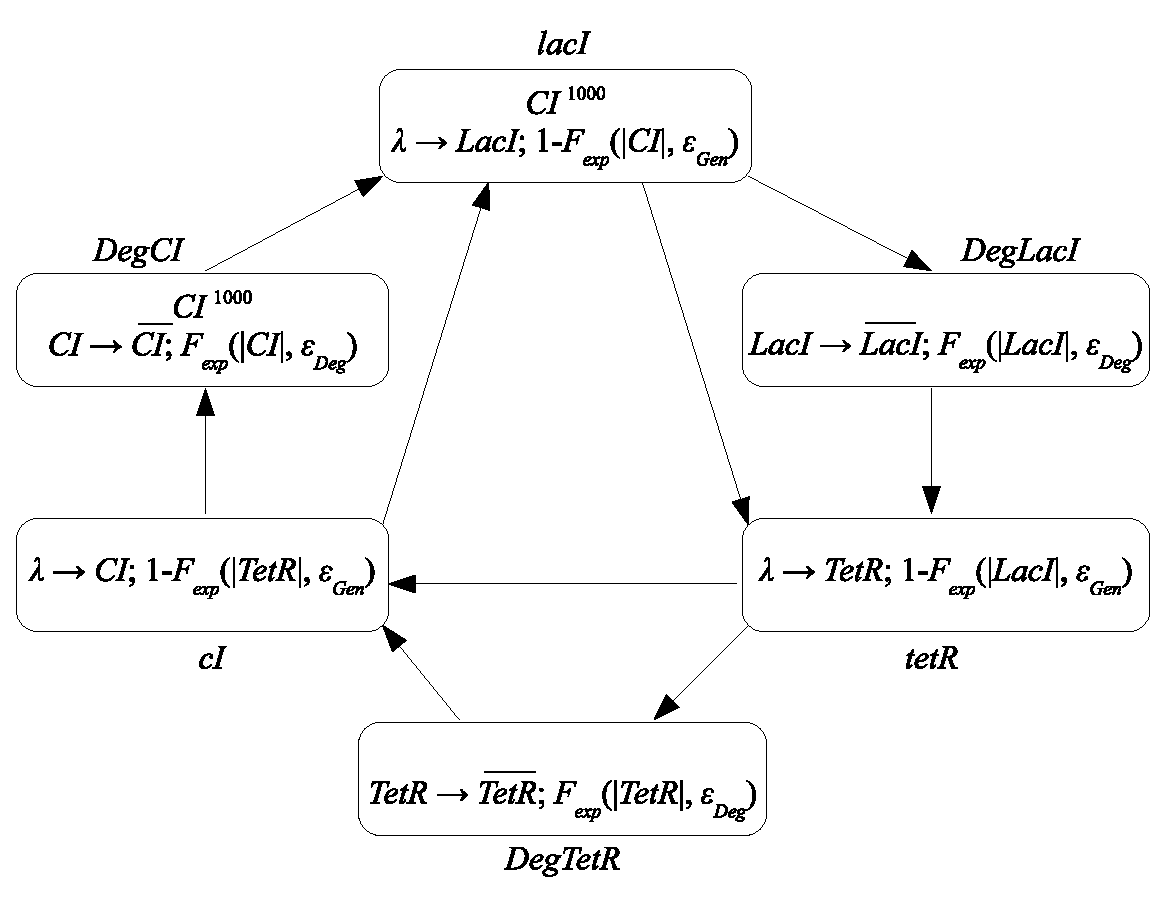
\includegraphics[width=0.67\textwidth]{DiagRepress}
\caption{The \textit{repressilator} model using BP system. Each of the three genes has an inhibitory effect on the next gene in the cycle. This is modelled by means of probability functions of the form $1-F_{exp}(..,..)$, which decreases the likelihood of the synthesis rule executing, the more inhibitor protein is present.}
\label{f:DiagRepress}
\end{center}
\end{figure}

The system is composed of three synthesis regions ---\textit{lacI}, \textit{tetR} and \textit{cI}--- connected with each other to form a ring, and their respective degradation regions ---\textit{DegLacI}, \textit{DegTetR} and \textit{DegCI}. The synthesis regions propagate copies of proteins by means of rules of the form $\lambda \rightarrow p_i; F_\sigma$, where $F_\sigma=1-F_{exp}(|p_j|, \epsilon_{Gen})$. Accordingly, as each gene has an inhibitory effect on the next one in the cycle, the more copies of the inhibitor protein $ p_j$ there are, the less likely the rule is to execute and therefore generate a copy of $p_i$. The degradation regions propagate anti-proteins of $p_i$ with a probability of $F_{exp}(|p_i|, \epsilon_{Deg} )$. The stability of the oscillations, the period of oscillation and the number of copies of each protein generated in each cycle can be controlled by the choice of parameters $\epsilon_{Gen}$ and $\epsilon_{Deg}$.

The model simulation shows that the system exhibits a stable and continuous oscillation, where all three genes, \textit{lacI}, \textit{tetR} and \textit{cI}, are activated one after the other in the order in which they appear in the cycle. Fig.~\ref{f:repress} shows the evolution of the number of copies of the proteins present in the system in two different simulations with parameters $\epsilon_{Gen} = 0.1$ and $\epsilon_{Deg} = 0.00125$ (Fig.~\ref{f:repress}a) and $\epsilon_{Gen} = 33.33$ and $\epsilon_{Deg} = 0.2$ (Fig.~\ref{f:repress}b). In the first case, we find that the oscillations are slow and the cycles long, but a lot of proteins are generated. In the second case, on the other hand, the oscillations are very fast (short cycles), but few proteins are generated. The two simulations differ as to how sensitive the regions are to the presence of proteins: they are less sensitive with $\epsilon_{Gen} = 0.1$ and $\epsilon_{Deg} = 0.00125$ (Fig.~\ref{f:repress}a) than with $\epsilon_{Gen} = 33.33$ and $\epsilon_{Deg} = 0.2$ (Fig.~\ref{f:repress}b), meaning that both synthesis and degradation are very slow, leading to longer oscillation cycles

\begin{figure}
\begin{center}
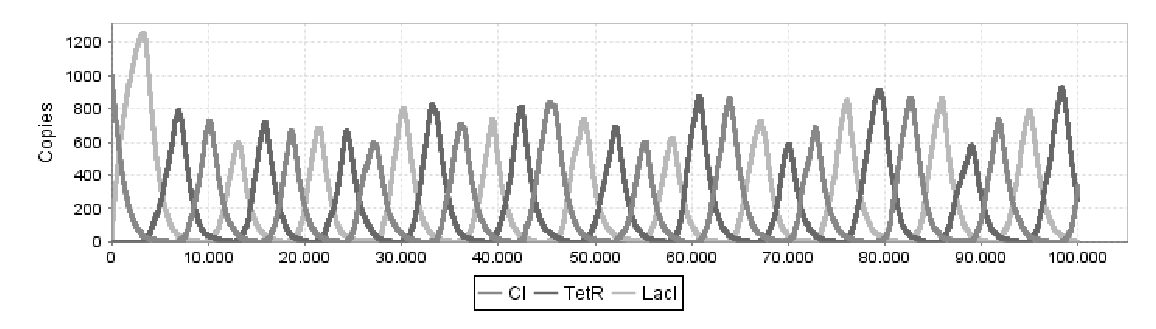
\includegraphics[width=1\textwidth]{repress1}
(a)
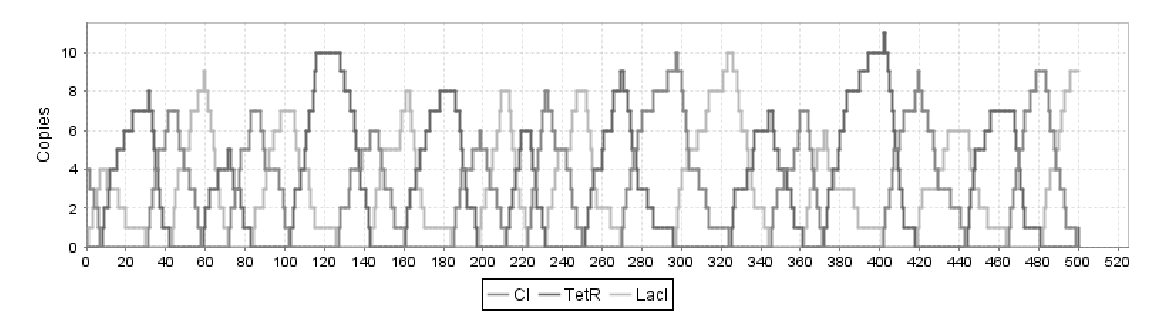
\includegraphics[width=1\textwidth]{repress2}
(b)
\caption{Two simulations of the \textit{repressilator} with parameters $\epsilon_{Gen} = 0.1$ and $\epsilon_{Deg} = 0.00125$ (a) and $\epsilon_{Gen} = 33.33$ and $\epsilon_{Deg} = 0.2$ (b). Small values of $\epsilon_{Gen}$ and $\epsilon_{Deg}$ (a) lead to long cycles generating a large quantity of proteins, whereas large values (b) make the system oscillate much faster generating fewer proteins.}
\label{f:repress}
\end{center}
\end{figure}

\begin{figure}
\begin{center}
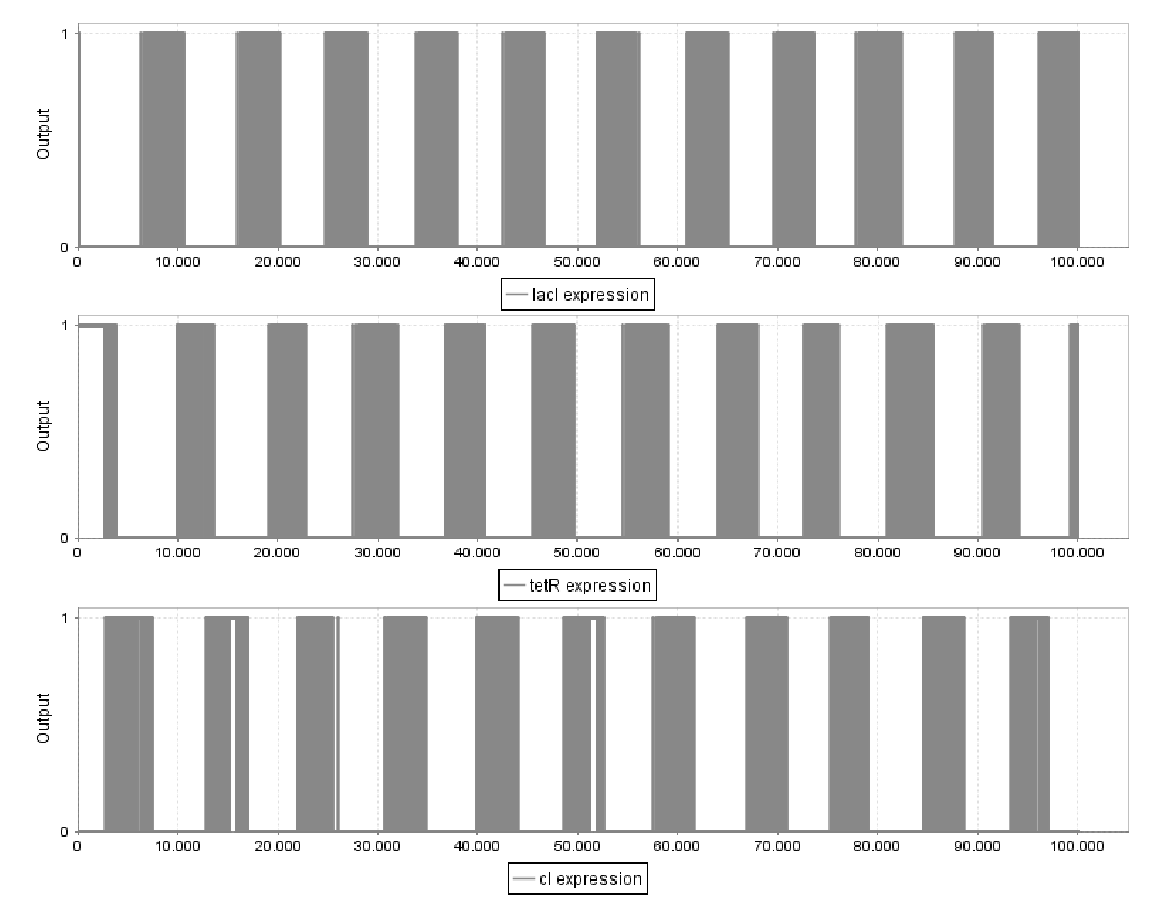
\includegraphics[width=1\textwidth]{sim}
\caption{Gene expression in the simulation with parameters $\epsilon_{Gen} = 0.1$ and $\epsilon_{Deg} = 0.00125$. There are successive periods of gene expression in the order in which the genes appear in the network, and the periods of expression are of similar duration and overlap with approximately the last third of the previous gene.}
\label{f:sim2}
\end{center}
\end{figure}

Fig.~\ref{f:sim2} also shows the system oscillation in the period of gene expression for the case of $\epsilon_{Gen} = 0.1$ and $\epsilon_{Deg} = 0.00125$: Genes exhibit very long periods of expression, of the order of 4000 simulation iterations, where iterations in which the synthesis rule is and is not executed alternate in frequent transitions from 0 to 1 and vice versa. Because of the transition frequency, the periods of expression are displayed as solid bars in the chart. Upon closer observation (see Fig.~\ref{f:detail}), however, it is apparent how the period of expression starts and ends gradually with sporadic protein propagations that steadily increase in frequency until they succeed each other continuously from iterations 81000 to 81750. They then slow down until they come to a complete standstill, and subsequently start up again in the next period of activity. In other words, when the expression intensity of one gene drops, the next gene starts to exhibit activity so that one gene is always being expressed.

\begin{figure}
\begin{center}
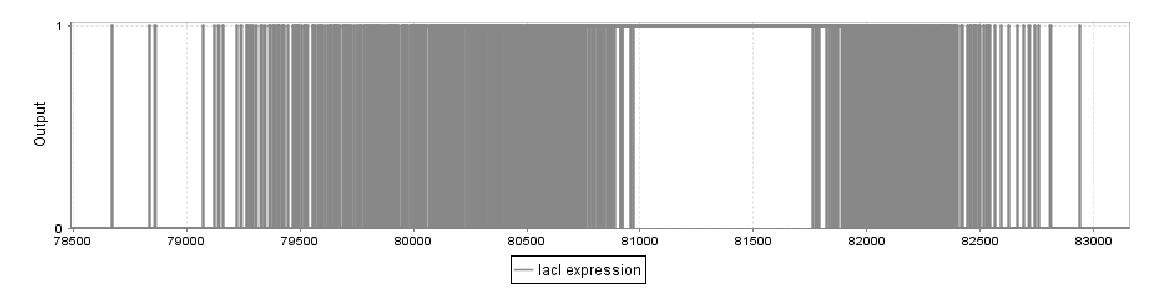
\includegraphics[width=1\textwidth]{detail}
\caption{Detail of the expression of \textit{lacI} in the simulation with parameters $\epsilon_{Gen} = 0.1$ and $\epsilon_{Deg} = 0.00125$ from iterations 78500 to 83000. As the inhibitory proteins \textit{CI} decrease (are degraded), the gene starts to be expressed, first sporadically and then gradually more and more often, stabilizing at 1 until approximately iteration 81750. At this point, copies of \textit{CI} arrive again and gradually start to inhibit gene expression.}
\label{f:detail}
\end{center}
\end{figure}
%
\section{Conclusions}
Bursting P systems are a feasible and realistic way of building qualitative models of genetic regulatory networks, as demonstrated by the \textit{repressilator} example presented as case study. These systems emulate the mechanism producing protein bursts in biological cells, using rules that are executed probabilistically depending on the number of copies of the regulatory proteins. Gene response to the presence of transcription factors is modelled by means of exponential probability distributions whose parameter regulates their sensitivity to the presence of copies of activator/inhibitor proteins. On the other hand, these same probability distributions are also used to model the exponential decay of the degrading proteins. In sum, the use of probability distributions enables the model to account for randomness, stochasticity, noise and fuzzy behaviour, as would be expected of a real system.


Although we have used exponential probability functions in this paper, it might be worthwhile to research the behaviour of these systems using other distribution functions in the future. Additionally, the model only accounts for the effect of transcription factors on the frequency of the bursts, all of which are of the same size, as the execution of a rule produces a single copy of a protein object. But, as suggested in~\cite{Raj2006}, it is conceivable that the presence of transcription factors might influence the amplitude (that is, the size) of those bursts rather than their frequency. Thus, it might be worthwhile examining how the system would work with rules like $\lambda \rightarrow p^r$, with $r \geq1$, where the number $r$ of copies of the protein $p$ produced would somehow, either deterministically or stochastically, be a function of the number of transcription factors. 

\bibliography{paper}{}
\bibliographystyle{plain}

\end{document}

